\subsection{Property View Models}


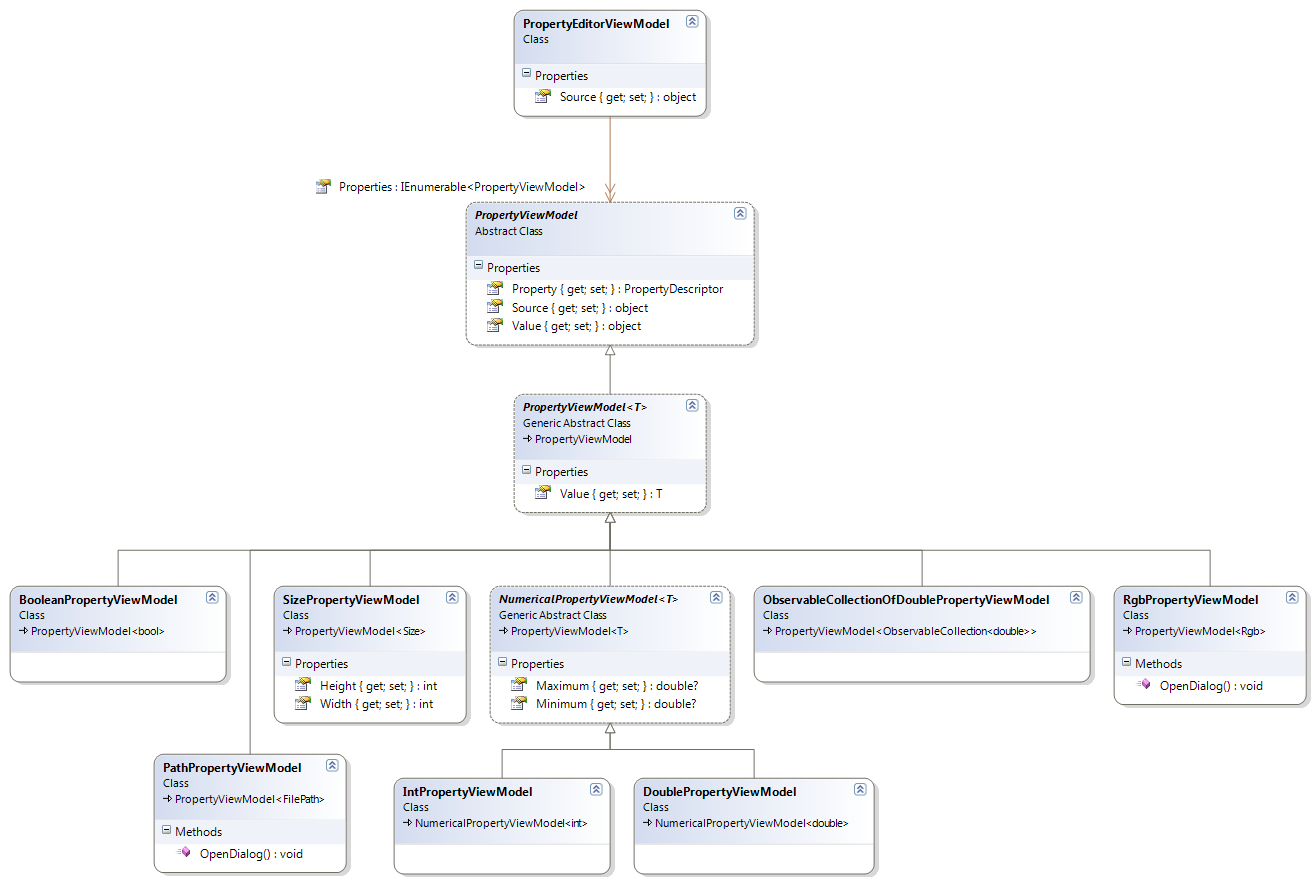
\includegraphics[width=\textwidth]{YuvKA.ViewModel.PropertyEditor/propertyEditor.png}
Diese Klassen dienen der Darstellung der vom Benutzer veränderbaren Properties unter Zuhilfenahme der View. 



\subsubsection{YuvKA.ViewModel.PropertyEditor.PropertyEditorViewModel}

\begin{verbatim}
public class PropertyEditorViewModel
\end{verbatim}

\paragraph{Beschreibung}~\\
Die Klasse \name{PropertyEditorViewModel} verwaltet eine Anzahl von Properties und ermöglicht mithilfe der View ihre Darstellung.

\paragraph{Typmember}
\begin{itemize}

\property{Properties}
	\begin{verbatim}
	public IEnumerable<PropertyViewModel> Properties { get; }
	\end{verbatim}
	Ruft die Liste der zu verwaltenden Properties ab.

\property{Source}
	\begin{verbatim}
	public object Source { get; }
	\end{verbatim}
	Ruft die Quelle der zu verwaltenden Properties ab.

\end{itemize}




\subsubsection{YuvKA.ViewModel.PropertyEditor.PropertyViewModel}

\begin{verbatim}
public abstract class PropertyViewModel
\end{verbatim}

\paragraph{Beschreibung}~\\
Abstrakte Oberklasse zu den einzelnen Property View Model Klassen

\paragraph{Typmember}
\begin{itemize}
 	
\property{Property}
	\begin{verbatim}
	public PropertyDescriptor Property { get; }
	\end{verbatim}
	Ruft die Beschreibung der verwalteten Property ab.

\property{Source}
	\begin{verbatim}
	public object Source { get; }
	\end{verbatim}
	Ruft die Quelle der verwalteten Property ab.

\property{Value}
	\begin{verbatim}
	public object Value { get; set; }
	\end{verbatim}
	Ruft den Wert der verwalteten Property ab oder legt ihn fest.

\end{itemize}




\subsubsection{YuvKA.ViewModel.PropertyEditor.PropertyViewModel\textless T\textgreater}

\begin{verbatim}
[InheritedExport]
public abstract class PropertyViewModel<T> : PropertyViewModel
\end{verbatim}

\paragraph{Beschreibung}~\\
Typisierte Ableitung der \name{PropertyViewModel}-Klasse

\paragraph{Typmember}
\begin{itemize}

\property{Value}
	\begin{verbatim}
	public T Value { get; set; }
	\end{verbatim}
	Ruft den Wert der Property ab oder legt ihn fest. T ist hierbei der Typ der verwalteten Property.
\end{itemize}



\subsubsection{PropertyViewModel-Implementierungen}

\begin{itemize}

\item{\textbf{YuvKA.ViewModel.PropertyEditor.BooleanPropertyViewModel}}
	\begin{verbatim}
	public class BooleanPropertyViewModel : PropertyViewModel<bool>
	\end{verbatim}
	Stellt mithilfe der View eine Property vom Typ \name{bool} dar.

\item{\textbf{VuvKA.ViewModel.PropertyEditor.PathPropertyViewModel}}
	\begin{verbatim}
	public class PathPropertyViewModel : PropertyViewModel<FilePath>
	\end{verbatim}
	Stellt mithilfe der View eine Property, welche einen Dateipfad darstellt, dar.\\
	Die Klasse besitzt zudem die folgende Methode, welche einen Dialog zur Auswahl des Dateipfades öffnet:
	\begin{verbatim}
	public void OpenDialog()
	\end{verbatim}

\item{\textbf{YuvKA.ViewModel.PropertyEditor.SizePropertyViewModel}}
	\begin{verbatim}
	public class SizePropertyViewModel : PropertyViewModel<Size>
	\end{verbatim}
	Stellt mithilfe der View eine Property vom Typ \name{Size} dar.\\
	Die Klasse besitzt folgende Properties, welche die Höhe und die Breite von \name {Size} repräsentieren:
	\begin{verbatim}
	public int Width { get; set; }
	public int Height { get; set; } 
	\end{verbatim}

\item{\textbf{YuvKA.ViewModel.PropertyEditor.NumericalPropertyViewModel}}
	\begin{verbatim}
	public abstract class NumericalPropertyViewModel<T> 
	: PropertyViewModel<T>
	\end{verbatim}
	Stellt mithilfe der View eine numerische Property dar. Die Klasse besitzt zudem die folgenden Properties, welche die obere und untere Grenze der darzustellenden Property darstellen:
	\begin{verbatim}
	public Nullable<double> Maximum { get; set; }
	public Nullable<double> Minimum { get; set; }
	\end{verbatim}
	Von dieser Klasse erben die folgenden numerischen Property View Models, welche einen \name{int}-Wert bzw einen \name{double}-Wert darstellen:

	\begin{verbatim}
	public class IntPropertyViewModel 
	: NumericalPropertyViewModel<int>
	
	public class DoublePropertyViewModel 
	: NumericalPropertyViewModel<double>
	\end{verbatim}				

\item{\textbf{YuvKA.ViewModel.PropertyEditor.ObservableCollectionOfDoublePropertyViewModel}}
	\begin{verbatim}
	public class ObservableCollectionOfDoublePropertyViewModel 
	: PropertyViewModel<ObservableCollection<double>>
	\end{verbatim}
	Stellt mithilfe der View eine \name{ObservableCollection} von \name{double}-Werten dar.

\item{\textbf{YuvKA.ViewModel.PropertyEditor.RgbPropertyViewModel}}
	\begin{verbatim}
	public class RgbPropertyViewModel : PropertyViewModel<VideoModel.Rgb>
	\end{verbatim}
	Stellt eine \name{Rgb}-Property mithilfe der View dar.\\
	Die Klasse besitzt die folgende Methode, welche einen Dialog zur Farbauswahl öffnet:
	\begin{verbatim}
	public void OpenDialog()
	\end{verbatim}

\end{itemize}


